\chapter{Typing Dependency Structure}
\label{chapter:chapter_2}

\chapabstract{
	``Predicates are functors,\\
	complements -- diamonds,\\
	adjuncts -- boxes;\\
	Everything a type.''
}

The previous chapter initiated us into the history-rich world of substructural logics in the intuitionistic tradition.
Along the (artificially homogenized) story, we got to dip our toes into linguistic waters, where we saw these logics thrive and prosper, finding their place as the foundation for categorial grammars.
The many flavours of categorial grammars all have a single common denominator: they treat syntax as a hierarchical structure that puts phrases together from small to big, starting from words and reaching up to the sentence, the imprint being a natural deduction tree (and perhaps a phrasal bracketing structure).
This emphasis on the phrase, combined with the distinctive shape of the categorial parse, allows for a partial parallel to be drawn between categorial grammars and phrase structure grammars, despite their stark methodological and theoretical contrasts.
These are rule-based systems that assign categories to phrases according to their syntactic function, and manipulate phrasal formation by specifying how their constituent parts combine -- the produce being a bracketing structure, commonly visualized in tree format.

A different approach to grammatical theory abandons constituency relation in favour of the dependency relation in its stead.
Dependency relations do not seem compatible with the categorial setup at a first glance: they are flat, and lack the notion of finite phrasal parts -- in showing no attachment to iterative phrasal division, they are also not obviously compositional.
In this chapter we will focus our efforts into bridging this gap between these two perspectives, under a unified categorial grammar setup.
We will motivate the incorporation of dependency relations into the categorial vocabulary by repurposing existing, well-studied tools that remain faithful to the formal logic and type theory roots the previous chapter has established.

\section{Phrase vs. Dependency Structure}
Before we get to theorycrafting, it would be useful to try and clarify what exactly is meant by constituency- and dependency-structure, and what the distinctions between the two are.

\subsection{Phrase Structure Grammars}
Phrase structure grammars build on the observation that certain phrases seem to act as rigid and independent chunks, sometimes referred to as \textit{constituents}. 
Viewed from within, these phrases may be rich in internal structure, but keep it sealed off to the outside.
Viewed externally (i.e. in the context of a wider phrase that contains them), they are indivisible units, or at least for the purposes of phrasal composition.
Phrases are inventorized according to their syntactic \textit{categories}.
If one so wishes, they can for the most part replace a phrase for another of the same category, with no effect to grammaticality or local structure, which suggests they are functionally indiscernible.
% \todo clarity
% us -> as, i.e. -> e.g.
For instance, the underlined phrases are interchanged among the examples below, keeping the outermost phrasal structure intact, despite their wildly different internal structures%
\footnote{Sourced from H.P. Lovecraft, \textit{Celepha\"{i}s}  (1922). In \textit{The Rainbow, vol. 2.}}:

{\smaller%
\begin{enumerate}
\item $\w{he}\sbind(\w{beheld}\sbind\underline{(\w{the}\sbind\w{city})})$
\item $\w{he}\sbind(\w{beheld}\sbind\underline{(\w{the}\sbind((\w{glittering}\sbind{\w{minarets}})\sbind(\w{of}\sbind(\w{the}\sbind\w{city}))))})$
\item $\w{he}\sbind(\w{beheld}\sbind(\underline{(\w{such}\sbind\w{beauty})\sbind(\w{of}\sbind((\w{red}\sbind(\w{and}\sbind\w{white}))\sbind\w{flowers})))})$
\item $\w{he}\sbind(\w{beheld}\sbind(\underline{
	(
		\w{some}\sbind
			(\w{feature}\sbind
				(\w{or}\sbind\w{arrangement})
			)\!\sbind\!
			(\w{which}\sbind
				(\w{he}\sbind
					(
						(\w{had}\sbind\w{known})\sbind
						\w{before}
					)					
				)
			)})$
\end{enumerate}}%

\noindent These so-called constituents interact, then, with one another depending not on their contents, but rather their categories.
This perspective promotes a disciplined approach to grammar modeling, dating back to the formal grammars of \citet{chomsky1956three}, the archetypical example being context-free grammars~\cite{chomsky1956three,jw1959c}.
There, the construction of complex expressions is guided by \textit{production rules}, grammatical recipes that dictate what categories can sequentially combine, in what order, and what the category of their combination is.
The above example would correspond, for instance, to production rules of the form:
\begin{align}
	S 	& 	\to NP \ VP \label{equation:sfromnpvp}\\
	VP 	&	\to TV \ NP \label{equation:vpfromtvnvp}
\end{align}
claiming that one of the ways to make a verb phrase $VP$ involves concatenating a transitive verb $TV$ with a noun phrase $NP$, which in turn can be plugged to the right of another $NP$ to produce a declarative sentence $S$ -- each rule leaving a bracketing structure (or binary tree) in its wake (see Figure~\ref{subfigure:cfgtree}).


\begin{figure}
	\centering
	\hfill%
	\begin{subfigure}[b]{0.35\textwidth}
		\begin{tikzpicture}
			\Tree 
				[ .{$S$} 
					[.{(\ref{equation:sfromnpvp})}
						[.{$NP$} 
							\w{he} 
						] 
						[.{$VP$}
							[.{(\ref{equation:vpfromtvnvp})} 
								[.{$TV$} \w{beheld} ] 
								[.{$NP$} 
									\edge[roof]; {\dots} 
								] 
							]
						] 
					]
				] 
		\end{tikzpicture}
		\caption{Context-free parse tree.}
		\label{subfigure:cfgtree}
	\end{subfigure}\hfill%
	\begin{subfigure}[b]{0.45\textwidth}
		\begin{tikzpicture}
			\Tree 
				[ .\s[s]
					[.{$\appleft$}
						[.{\np[s]}
							\w{he}
						]
						[.{$\np[s]\divleft\s[s]$}
							[.{$\appright$}
								[.{$(\np[s]\divleft\s[s])\divright\np[s]$} \w{beheld} ]
								[.{\np[s]}
									\edge[roof]; {\dots}
								]
							]
						]
					]
				]
		\end{tikzpicture}
		\caption{Tree-formatted Lambek derivation.}
		\label{subfigure:lambektree}
	\end{subfigure}\hfill
	\caption{A phrase-structure grammar parse tree (left) contrasted with a Lambek abstract syntax tree (right).}
	\label{figure:cfgvslambek}
\end{figure}

Even though context-free grammars are no longer seriously considered in the linguistic world, they have directly influenced most early attempts at grammar design -- and by extension, their later successors and refinements.
Notational evidence of this past are more than noticeable today, ranging from the wide adoption of tree-style notation for syntactic analyses to the conceptual syncretism of constituency grammars and phrase structure ones.
More up-to-date frameworks expand upon the barebones context-free backend with niceties like a distinction between functional dominance and linear precedence, added rules that manipulate movement and discontuinity, the proclamation of a single category as the \textit{head} of a production rule (or subtree), feature markings that carry semantic, morphological or phonological information, incorporation of dependency information, etc.~\cite[\textit{inter alia}]{gazdar1985generalized,jacobson1987phrase,pollard1994head,dalrymple2001lexical}.

To our ill fortune, the field of formal syntax is actually an informal mess, more akin to a mine field rather than an academic one; it's best if I don't overextend myself here, in order to avoid setting off unseen traps or causing easily avoidable confusion.
The point I want to make is that the focal center of the above formalisms is the \textit{phrase} and its structure -- as such, they are all referred to as phrase structure grammars, regardless of whatever extra fluff they carry or what their expressive capacity is.
In that broader sense of the term, and removing any implicit connotations of intellectual lineage, categorial grammars can also be conceived as phrase-centric.
Pure Lambek systems, for one, also explicate how phrases are combined, adhere to hierarchical forms similar to those of context-free grammars (except beautifully, see Figure~\ref{subfigure:lambektree}), and have the exact same expressive capacity~\cite{pentus1993lambek}.
They abstract away from the rule inventory by utilizing the smallest and purest set of rules possible -- those of function application and variable abstraction -- and internalize what used to be rule-imposed structure within the lexical categories themselves.
Bracketing structure is now the footprint of function application, and the interface with semantics is naturalized by virtue of the Curry-Howard correspondence, as we saw earlier.
Rather than a $VP$ category and rule~(\ref{equation:sfromnpvp}), we have the \textit{type} $\np[s]\divleft\s[s]$ -- transparent with respect to both its syntactic combinatorics and semantic function.
Performing the function application on a left-adjacent \np[s] will then result to a local tree structure, not unlike the corresponding production rule -- see Figure~\ref{figure:cfgvslambek} for a comparison.
Note that in reality, categorial derivations in the type-theoretic tradition resemble trees only locally, since in high-order phenomena involving abstractions the unary, non-terminal $\lambda$ nodes will either need to be uniquely named with the variable they are binding, or otherwise point to it  with an additional edge -- hence a directed acyclic graph could make for a more accurate representation format.
Long story short, even without extensions to the logical core for managing discontuinity, calling deductive parsing constituency parsing would obviously not be doing the former justice; yet despite their methodological and theoretical divergences, their end yield is comparable -- the antecedent structures of Figures~\ref{figure:nl_applicative_examples} to~\ref{figure:lovecraft_coord} testify that the former may in fact be seen as subsuming the latter.

\subsection{Dependency Grammars}
The constituency tradition has co-evolved along the opposing view of dependency grammars~\cite[\textit{inter alia}]{sgall1986meaning,mel1988dependency,sleator1995parsing}.
Dependency grammars reject the binary phrasal division that constituency grammars abide by, and instead adopt a flatter structural form, the only unit of which is the word.
Words are connected with one another by dependency arcs, i.e. directed edges between word pairs.
Each word can have arbitrarily many outgoing edges (dependents), but only a single incoming edge (head) -- the exception is the root word which has no head of its own (i.e. the head of the matrix clause).
This articulation of a distinction between heads and dependents is central to dependency grammar.
In a semantically-oriented extension, edges can be assigned an extra direction that needs not agree with the syntactic one, pointing instead from semantic predicate to semantic argument~\cite{mel2003levels}.
A word is said to directy dominate its dependents, and indirectly dominate all words its dependents dominate (directly or otherwise) -- e.g. the root indirectly dominates every other word in the sentence.
The dependency structure of a sentence is once more a tree, with words now as both terminal and non-terminal nodes, glued together with dependency relations.
A dependency tree is uncostrained by adjacency and word order: edges can penetrate or fly over other edges.
This perspective is computationally appealing due to its simplicity and uniformity, as it allows a dependency grammar to argue about languages with wildly diverging syntactic and typological properties while remaining virtually unchanged.
For the exact same reasons, it can also be seen as concealing -- it sacrifices any potential of targeted analysis in the pedestal of universality.

A dependency grammar that has gained significant traction over the last decade is the framework of universal dependencies~\cite{10.1162/coli_a_00402}, boasting a vast multi-lingual collection of treebanks~\cite{nivre2020universal} and tools.
In the universal dependencies framework, dependency relations are labeled according to their grammatical function, allowing the distinction of a words' dependents according to the grammatical role they fulfill.
Grammatical roles are typologically and thematically informed, and are inventorized with language universality as the prime goal.
From a semantic point-of-view, these roles can also be seen as specifying whether semantic flow is co- or contra-directional to syntactic flow, i.e. whether a dependency marks a complement (where syntactic head and semantic predicate coincide) or an adjunct (where the syntactic head is the semantic argument of its syntactic dependent).
On top of the labeled arcs, words are usually assigned a label pulled from a rudimentary set of part of speech tags and lexical identifiers.

\begin{figure}
	\centering
	\begin{tikzpicture}[t/.style={text height=1.5ex, text depth=.25ex, rectangle, outer sep=0pt}, node distance=10pt]
	\smaller
	\node[t] (he) 			at (0, 0) {\w{he}};
	\node[t] (he_)			[below=4pt of he] {\w{PRON}};
	\node[t] (beheld)		[right=10pt of he] {\w{beheld}};
	\node[t] (beheld_)		[below=4pt of beheld] {\w{VERB}};
	\node[t] (the) 			[right=10pt of beheld] {\w{the}};
	\node[t] (the_)			[below=4pt of the] {\w{DET}};
	\node[t] (glittering) 	[right=10pt of the] {\w{glittering}};
	\node[t] (glittering_)	[below=4pt of glittering] {\w{VERB}};
	\node[t] (minarets)		[right=10pt of glittering] {\w{minarets}};
	\node[t] (minarets_)	[below=4pt of minarets] {\w{NOUN}};
	\node[t] (of)			[right=10pt of minarets] {\w{of}};
	\node[t] (of_)			[below=4pt of of] {\w{ADP}};
	\node[t] (the2)			[right=10pt of of] {\w{the}};
	\node[t] (the2_)		[below=4pt of the2] {\w{DET}};
	\node[t] (city)			[right=10pt of the2] {\w{city}};
	\node[t] (city_)		[below=4pt of city] {\w{NOUN}};
	\draw[->] (beheld) [bend right=80] edge node [above] {\smaller[2]{nsubj}} (he);
	\draw[->] (beheld) [bend left=90] edge node [above] {\smaller[2]{dobj}} (minarets);
	\draw[->] (minarets) [bend right=40] edge node [above] {\smaller[2]{amod}} (glittering);
	\draw[->] (minarets) [bend right=70] edge node [above] {\smaller[2]{det}} (the);
	\draw[->] (minarets) [bend left=60] edge node [above] {\smaller[2]{prep}} (of);	
	\draw[->] (of) [bend left=90] edge node [above] {\smaller[2]{pobj}} (city);	
	\draw[->] (city) [bend right=60] edge node [above] {\smaller[2]{det}} (the2);
	\end{tikzpicture}
	\caption{A sample dependency parse in the universal dependencies format.}
	\label{figure:udparse}
\end{figure}

Figure~\ref{figure:udparse} shows an example dependency parse.
Unlike before, we can not claim any semblance to the proofs that have occupied us thus far.
At a first glance, dependency grammars have little in common with categorial grammars -- structures are no longer binary nor made out of phrases, the axis of grammatical functions is competely new, and there seems to be little there reminiscent of the notions of induction and composition.
Though on closer inspection and armed with some goodwill, we can recover from some of these divergences if we make a few concessions from both sides.
We can start by treating any collection of words rooted in the same ancestor in the dependency graph as a constituent phrase, albeit possibly discontinuous -- the result will give as at least some partial overlap with the categorial directive.
Grammatical functions can then be thought of as being implicit, having been internalized in their positioning within a functor.
For instance we do intuitively know that the Lambek transitive verb $(\np[s]\divleft\s[s])\divright\np[s]$ requires an \textit{object} $\np[s]$ to the right and a \textit{subject} $\np[s]$ to the left -- marking them as such is perhaps redundant, since the verbal meaning recipe places each syntactic argument into a distinct semantic slot.
The binary bracketing structure is irrevocably lost, but this loss can be deemed as inconsequential if we ``flatten'' functor-induced phrasal boundaries by considering them only at these intermediary points where all of their arguments (however many) have been applied.
It is not much further we can get with this mediatory role, though.
No concession from the categorial side would be able to justify the absence of higher-order phenomena in a dependency graph,
and no concession from the dependency side could make peace with the absence of a head vs. predicate distinction of an applicative natural deduction proof.


\section{Modalities for Dependency Demarcation}
In our new quest, we will seek to design a type logic that subsumes and rises above both phrase structure grammars and dependency grammars.
As we saw in the previous section, the bar is not set particularly high for the first kind; the Lambek calculus can already do more than well enough.
The challenge then is to integrate the added values of a dependency grammar in a type-theoretic framework.
There's two elements we are missing; distinguishing between syntactic heads and semantic predicates, and marking words and phrases according to their grammatical roles within some wider context.

\subsection{Two Dimensional Predicates}
Categorial grammars are inherently and by design biased towards predicate structures, which is what after all makes them appealing for semantic use.
Each phrase can be iteratively split apart into two subphrases (not necessarily contiguous), where one provides a syntactic function, and the other the argument thereof.
Note that this distinction does not preclude the possibility that the argument itself has the shape of a function -- no assumption is made on the form of either subphrase's type, other than the two being compatible.
Higher-order syntactic phenomena in fact require that an incomplete phrase (i.e. a function) is supplied as the argument to another (i.e. a higher-order function, a function over functions).
But what constitutes a syntactic function in a local domain needs not always be the syntactic head of that domain.
There's a plethora of example cases.
Quantifiers, for instance, are inarguably functions over the objects they quantify, yet they exactly obey the morphosyntactic characteristics prescribed by these objects (i.e. grammatical gender, case, number, etc.), evidencing that the latter are in fact the heads -- a clear violation of the predicate/head alignment.
A similar argument can be made for determiners and, more broadly speaking, any element that is syntactically optional but semantically loaded, i.e. adjectival and adverbial modifiers.

\todo
This observation gives rise to a ... added dimension (2 with direct)
%Archeological excavations reveal that the first 

\bibliographystyle{abbrvnat}
\bibliography{bibliography}